  %%%%%%%%%%%%%%%%%%%%%%%%%%%%%%%%%%%%%%% -*- coding: utf-8; mode: latex -*- %%
  %
%%%%%                       CHAPTER
 %%%
  %

% $Id: 3100-nihil-molestiae.tex,v 1.1 2007/11/23 09:52:43 david Exp $
% $Log: 3100-nihil-molestiae.tex,v $
% Revision 1.1  2007/11/23 09:52:43  david
% *** empty log message ***
%
%

  %%%%%%%%%%%%%%%%%%%%%%%%%%%%%%%%%%%%%%%%%%%%%%%%%%%%%%%%%%%%%%%%%%%%%%%%%%%%%
  %
%%%%%                    HEAD MATTER
 %%%
  %

\chapter{Design and Implementation}
%\addcontentsline{lof}{chapter}{\thechapter\quad Nihil Molestiae}
%\addcontentsline{lot}{chapter}{\thechapter\quad Nihil Molestiae}
\label{ch:Design}

\section{Resolving the Semantic Related Group}

Resolving the semantic related group for each transaction is the fundamental step to preclude \textit{anomalies} in our implementation. The constraint between individual data is formed within a semantic related group. In Hop-HDFS, each metadata operation is implemented as an individual transaction running by a worker thread. Any metadata operation related to the namespace will have one or two input parameters, called \textit{Path}. Here's two examples for methods in the Filesystem API:

\begin{itemize}[noitemsep]
	\item boolean \textbf{mkdirs} (Path \textit{f}): \textit{f} is the path of the INodeDirectory to be created
	\item boolean \textbf{rename} (Path \textit{src}, Path \textit{dst}): \textit{src} is the path to be renamed, \textit{dst} is the new path after rename
\end{itemize} 

\noindent Each \textit{Path} object is related to a string representation of the "/" based absolute path name. For example, in Figure~\ref{fig:hoptree}, the path for INode \textit{h} is: 
\begin{center}
	/a/d/f/h
\end{center}

\noindent Therefore, with the preservation of the \textit{directed tree structure}, we can resolving a semantic related group for each INode along the edge of ancestors as a \textit{LinkedList}. The semantic related group representation for INode \textit{h} is:
\begin{center}
	h: \{/-$>$a-$>$d-$>$f\}
\end{center}

\noindent In other words, when mutating INode \textit{h}, all the semantic constraint can be found within INodes \textit{/, a, d, f}. With this knowledge, we can maintain the strung consistency semantics of original HDFS.

\noindent For each row in \textit{inodes table}, we can figure out its semantic related rows as shown in Table~\ref{table:semanticrelatedTable}.

\begin{table}[h]
	\centering
	\begin{tabular}{|c|c|c|c|c|}
		\hline
		~ & \textbf{id} & \textbf{parent\_id} & \textbf{name} & \textbf{other parameters...} \\ \hline
		Related * & 1 & 0 & / & ... \\ \hline
		Related * & 2 & 1 & a & ... \\ \hline
		~ & 3 & 1 & b & ... \\ \hline
		~ & 4 & 1 & c & ... \\ \hline
		Related * & 5 & 2 & d & ... \\ \hline
		~ & 6 & 3 & e & ... \\ \hline
		Related * & 7 & 5 & f & ... \\ \hline
		~ & 8 & 6 & g & ... \\ \hline
		Selected \checkmark & 9 & 7 & h & ... \\ \hline
		~ & 10 & 7 & i & ... \\ \hline
	\end{tabular}
	\caption{Table Representation for the Semantic Related Group}
	\label{table:semanticrelatedTable}
\end{table}   
  %%%%%%%%%%%%%%%%%%%%%%%%%%%%%%%%%%%%%%%%%%%%%%%%%%%%%%%%%%%%%%%%%%%%%%%%%%%%%
  %
%%%%%                      SECOND SECTION
 %%%
  %

\section{Per-Transaction Snapshot Isolation}

As we mentioned before, MySQL Cluster supports only the READ COMMITTED transaction isolation level, which means that the committed results of write operations in transactions will be exposed by reads in other transactions. Within a long running transaction, it could read two different versions of data, known as \textit{fuzzy read}, and it could also get two different sets of results if the same query is issued twice, known as \textit{phantom read}.

\noindent \textit{Snapshot isolation} guarantees that all reads made within a transaction see a consistent view of at the database. At the beginning of the transaction, it reads data from a snapshot of the latest committed value. During transaction execution, reads and writes are performed on the this snapshot.

\noindent In commercial database management systems, like Microsoft SQL Server, Oracle, etc, \textit{snapshot isolation} is implemented within multi version concurrency control (MVCC)~\cite{berenson1995critique} on database server side. However, we need to implement snapshot isolation on the application side since MySQL Cluster supports only the READ COMMITTED isolation level.

\noindent After resolving the semantic related group, we take a snapshot on selected rows as well as all related rows on the committed values from database. This snapshot will be cached in its transaction. Each transaction will have its own copy of snapshot during its lifetime. All transaction operations will be performed on its own snapshot. Therefore, we called it Per-Transaction Snapshot Isolation.

\noindent Before validation phase, the transaction will never fetch any data from database since it has all the semantic related rows in the cache. Therefore, the snapshot provides a consistent view of data for each transaction from read phase until validation phase: 
\begin{itemize}[noitemsep]
	\item \textit{Fuzzy Read} is precluded by \textit{snapshot isolation}: As we can see from Figure~\ref{fig:snapfuzzy}, the second read of Transaction 1 read from snapshot instead of database, not affected by the value committed by Transaction 2.
	\item \textit{Phantom Read} is also precluded by \textit{snapshot isolation with Semantic Related Group}: As we can see from Figure~\ref{fig:snapphantom}, Transaction 1 snapshot the semantic related group of x after the first count operation. So its second count operation is not affected by the value inserted by Transaction 2.
\end{itemize} 

\begin{figure}[h]
	\centering
	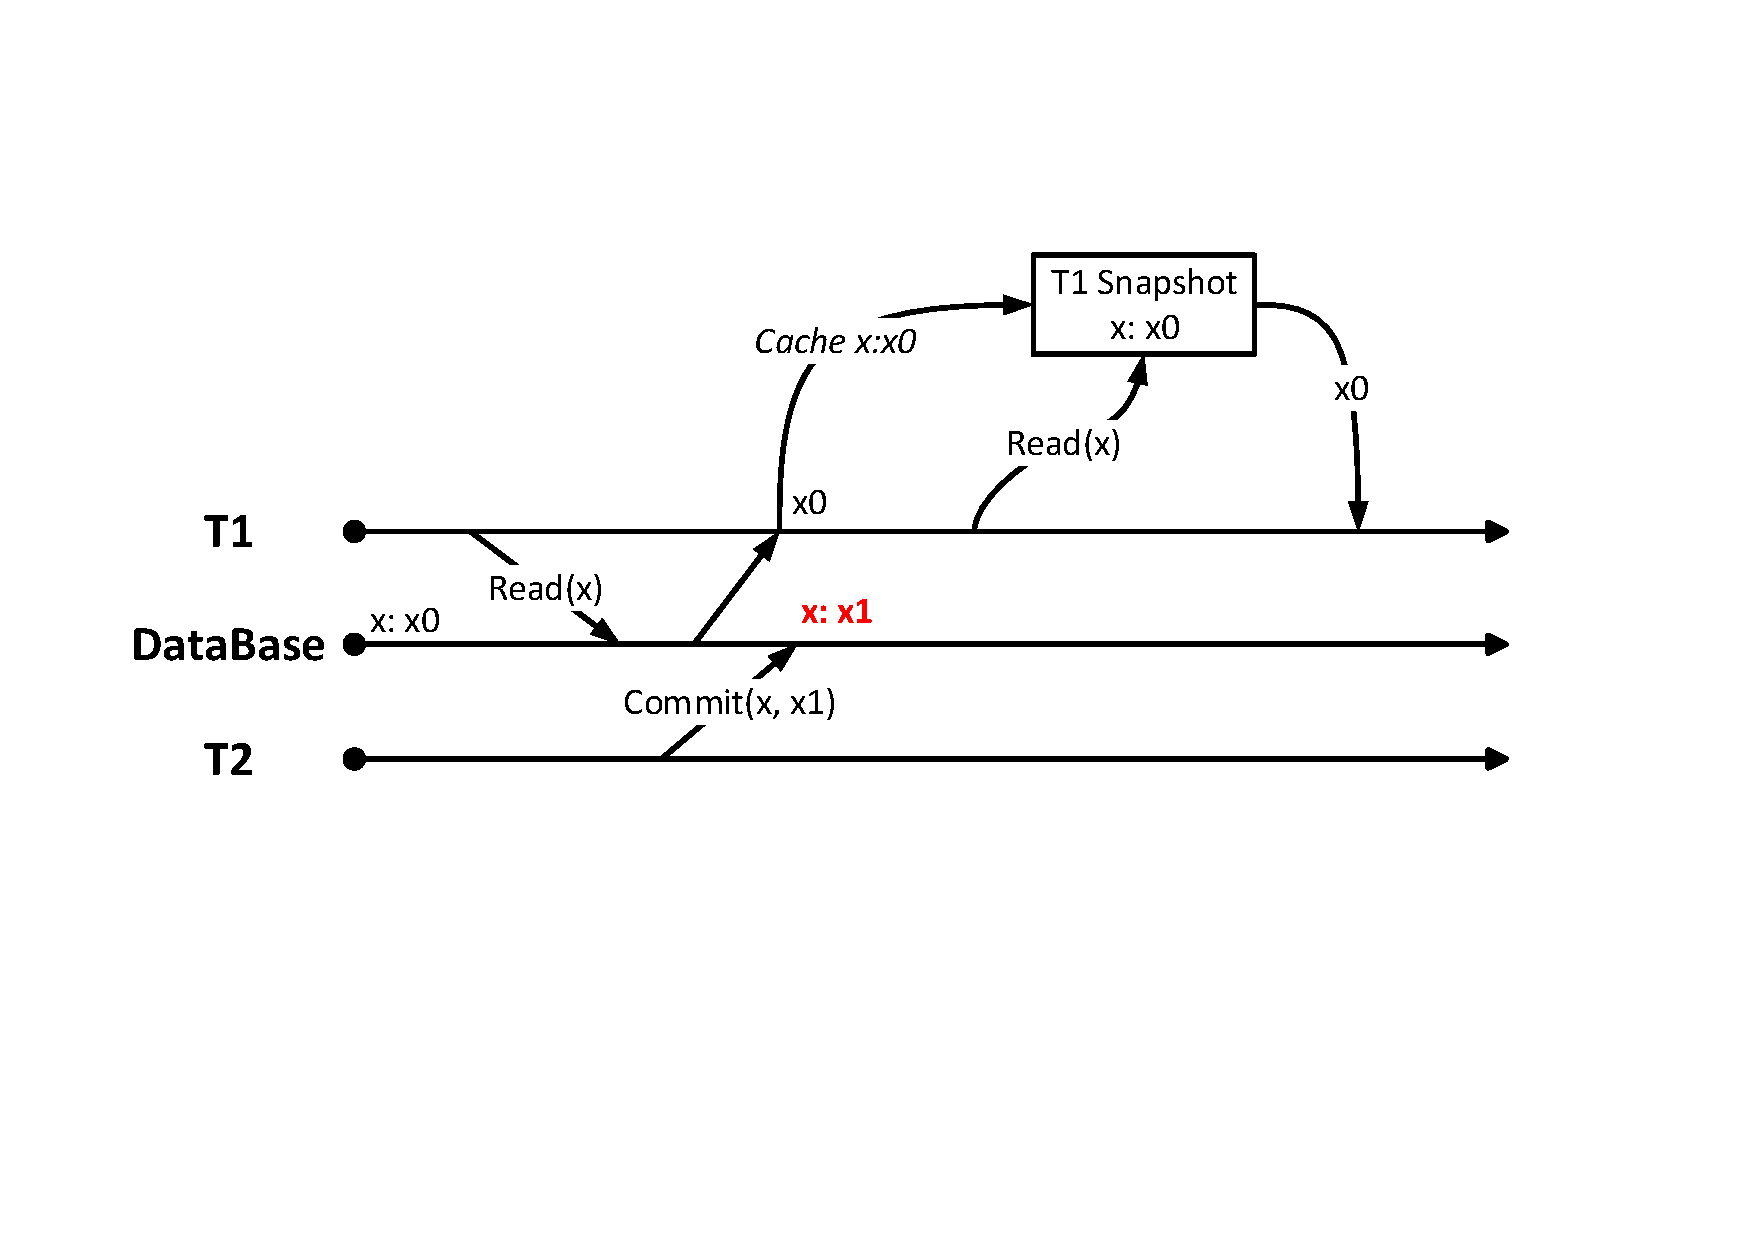
\includegraphics[width=\linewidth]{figs/snapfuzzy.pdf}
	\caption{Snapshot Isolation Precludes Fuzzy Read}
	\label{fig:snapfuzzy}
\end{figure}

\begin{figure}[h]
	\centering
	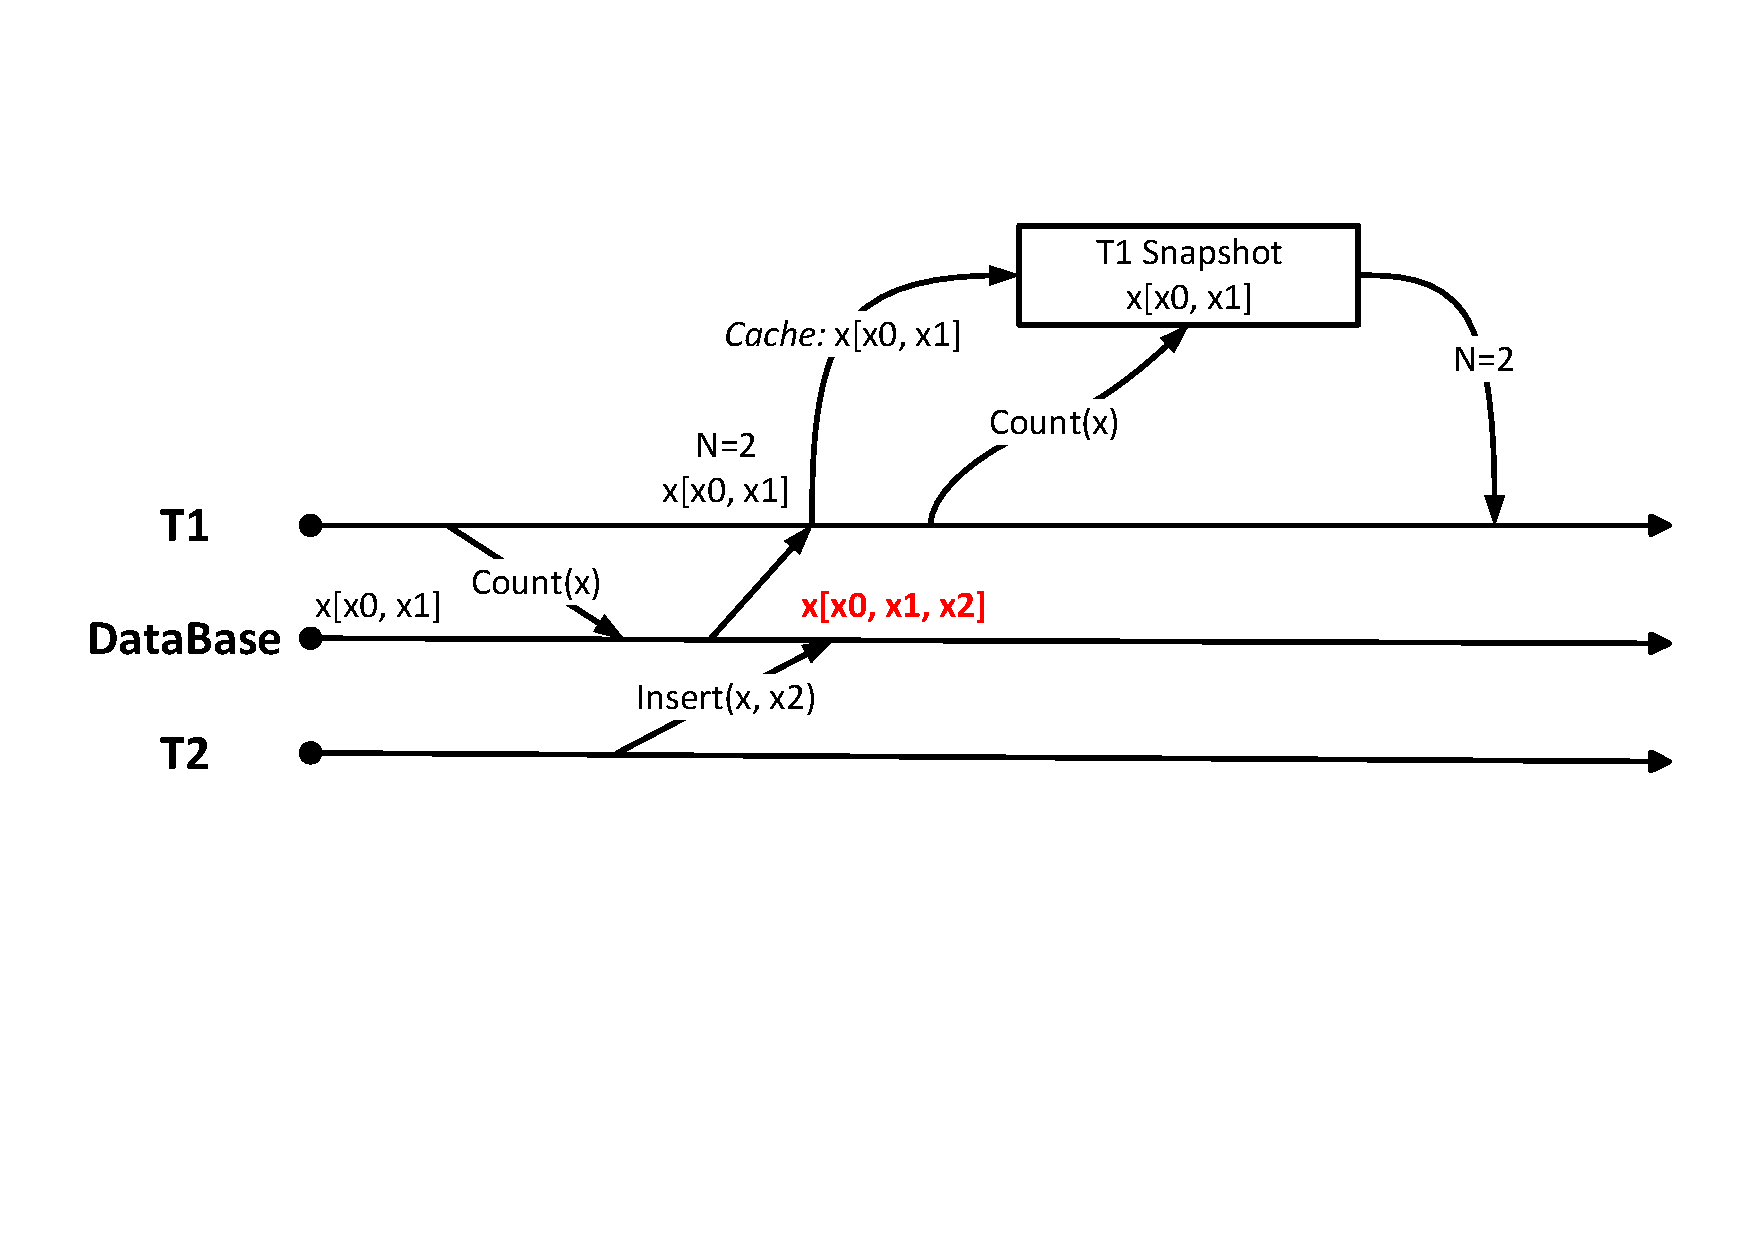
\includegraphics[width=\linewidth]{figs/snapphantom.pdf}
	\caption{Snapshot Isolation + Semantic Related Group Precludes Phantom Read}
	\label{fig:snapphantom}
\end{figure}
  %%%%%%%%%%%%%%%%%%%%%%%%%%%%%%%%%%%%%%%%%%%%%%%%%%%%%%%%%%%%%%%%%%%%%%%%%%%%%
  %
%%%%%                         ANOTHER SECTION
 %%%
  %
\section{C}

CCC

